\documentclass[12pt,notitlepage,nofootinbib]{revtex4}
\usepackage{graphicx}
\usepackage{bm}
\usepackage{rotating}
\def\baselinestretch{1.2}
\usepackage{dcolumn}
\usepackage{times}
\usepackage{color}
\usepackage{amsmath,amssymb,amsfonts} 
\usepackage{extarrows}
\usepackage{listings}
\usepackage{url}
\setlength{\mathindent}{0pt}

\begin{document}

\title{StochSS Hands-on Tutorial Series: 6 - Cloud Computing with StochSS}

\author{StochSS Development Team}
\affiliation{Department of Computer Science - University of California, Santa Barbara}

\date{\today}

\maketitle

\section{\label{sec:pre}Prerequisites}
\begin{itemize}
\item StochSS 1.5 (or later) installed on your computer (please follow download and installation instructions at \url{www.stochss.org}). 
\item A basic knowledge of the functionalities in the StochSS GUI (please consult the \textit{Basic Introduction to StochSS} tutorial).
\item The following login screen appears in your browser; please log in.
\end{itemize}


\begin{figure}[!ht]
\centering
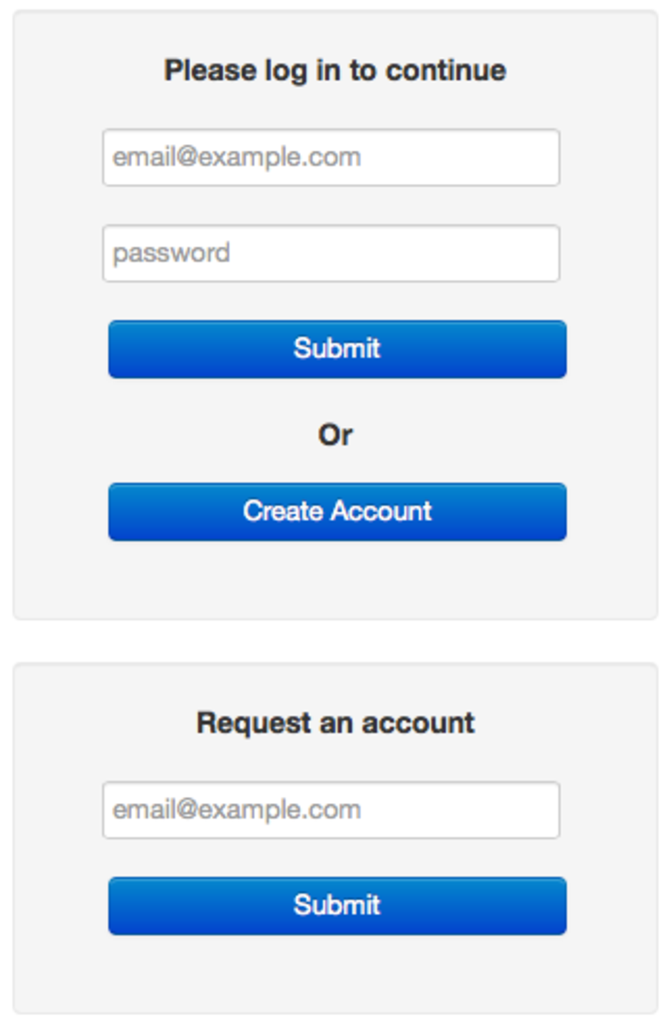
\includegraphics[scale=0.55]{user-login.pdf}
\end{figure}

\newpage

\section{Credentials}
StochSS provides the options to run different types of jobs using the cloud infrastructures. In StochSS 1.2-1.5, the cloud services it has are all by Amazon Web Service (AWS). In order to use AWS Elastic Computing Cloud (EC2), Simple Storage Service (S3) and DynamoDB database, which are all required by running jobs in the cloud, you should be prepared to have at least one AWS account and one credential (key pair) in hand. 

More information regarding how to create an AWS account or a security credential can be found here: \url{http://aws.amazon.com}

\subsection{An Instructive Example on Setting Credentials}
The StochSS will validate the credentials you to run job in the cloud. 

An example will be shown to you on how to validate your credentials in StochSS through the following steps:

\begin{figure}[!ht]
\centering
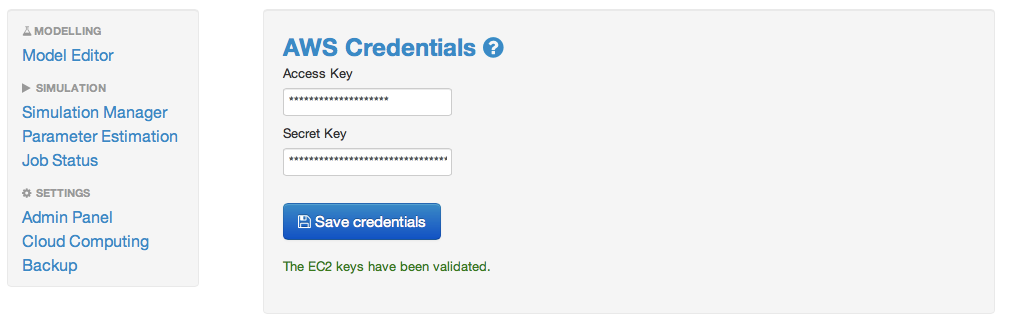
\includegraphics[scale=0.45]{T6_fig_credentials.png}
\caption{'Cloud Computing' page - 'Credentials' section}
\label{fig:2}
\end{figure}

\begin{itemize}
\item \textbf{Navigate} to the main \textcolor{blue}{Cloud Computing} page by \textbf{clicking} the ``Cloud Computing' on the side bar.
\item \textbf{Type in} or \textbf{copy} the access key id of your credentials in \textcolor{blue}{'Access Key'} text box.
 \item \textbf{Type in} or \textbf{copy} the secret access key of your credentials in \textcolor{blue}{`Secret Key'} text box. 
 \item \textbf{Click} on the \textcolor{blue}{'Save credentials'} button to save your credentials into the database. Whenever there is no computing node running (the nodes can be seen in the 'Status of VMs' section down the same page) with your current credentials, you could always change your credentials to another and save to restore them.
 \item \textbf{Double check} the credentials are valid by seeing the message below.

\end{itemize}

\newpage

\section{Compute Node}
There are as many as six different types of AWS EC2 compute nodes for you to run your jobs in the cloud: t1.micro, m1.small, m3.medium, m3.large, c3.large, c3.xlarge. These nodes comprise varying combinations of CPU, memory, storage, and networking capacity. Please follow the link to know more about different types of nodes: \url{http://aws.amazon.com/ec2/instance-types/}.

More information regarding how to create an AWS account or a security credential can be found here: \url{http://aws.amazon.com}

\subsection{An Example on Launching and Shutting Down Nodes}
Computing node section provides the options of both launching a default node and manually choosing combinations of different nodes at a time. In addition, the status of each launching node can be checked by refreshing the page. Moreover, there is only one click to terminate all running/pending/creating nodes.

An example will be shown on how to launch and shut down nodes as well as refresh the status:

\begin{figure}[!ht]
\centering
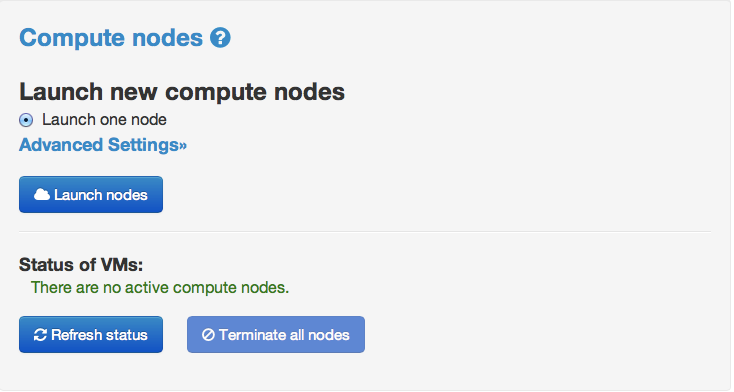
\includegraphics[scale=0.45]{T6_fig_computenode1.png}
\caption{'Cloud Computing' page - 'Compute nodes' default setting section}
\label{fig:2}
\end{figure}

\begin{itemize}
\item \textbf{Navigate} to the main \textcolor{blue}{Cloud Computing} page by \textbf{clicking} the 'Cloud Computing' on the side bar. \textcolor{blue}{Compute nodes} section is right below the \textcolor{blue}{Credentials}
\item 'One compute node at a time' is chosen by default, which means that you could \textbf{Click} \textcolor{blue}{'Launch nodes'} button directly and that will launch one c3.large node for you for the first time (as a head node) and all t1.micro nodes for the rest.
\item By \textbf{clicking} the \textcolor{blue}{'Refresh status'} button, you are able to check the status of the launching nodes.
\item By \textbf{clicking} the \textcolor{blue}{'Terminate all nodes'} button, you are able to terminate all nodes of all status. 

\end{itemize}

\begin{figure}[!ht]
\centering
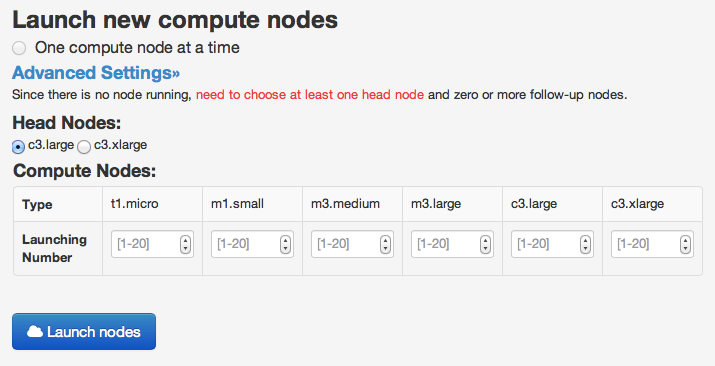
\includegraphics[scale=0.45]{T6_fig_computenode2.png}
\caption{'Cloud Computing' page - 'Compute nodes' advanced setting section}
\label{fig:2}
\end{figure}

\begin{itemize}
\item If you need more options on node types, \textcolor{blue}{'Advanced Settings'} will be the right place to take things under control.
\item \textbf{Choose} one of the \textcolor{blue}{'c3.large'} or \textcolor{blue}{'c3.xlarge'} if there is no head node running.
\item \textbf{Input in} more numbers in the text box under the proper types
\item \textbf{Click} the \textcolor{blue}{'Launch nodes'} button to launch the nodes you have chosen previously.

\end{itemize}

\newpage

\section{Reproduction}
To repeatedly access the output of a cloud job, StochSS provides the flexibility to both store the output in the cloud or reproduce the job every time it's needed (in order for less storage cost). By figuring out which way is the most economic for both time and money cost, you are encouraged to choose the better way of accessing the output.

\subsection{An Example on Job Reproduction}
An example shown below will guide you on how to reproduce a existing job.

\begin{figure}[!ht]
\centering
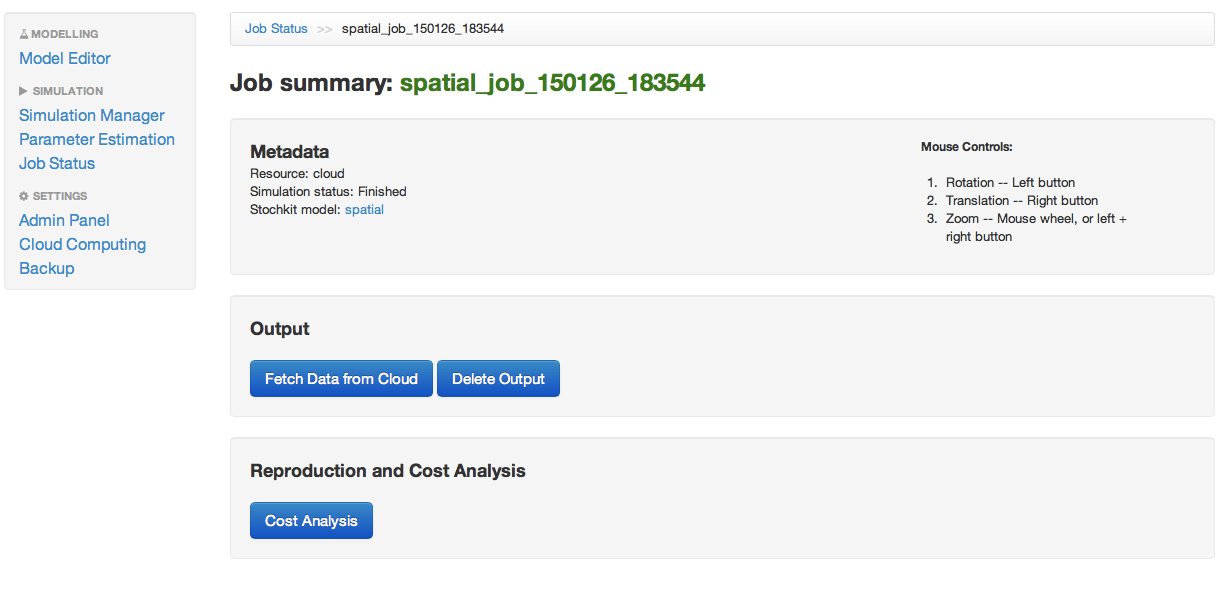
\includegraphics[scale=0.35]{T6_fig_reproduction2.png}
\caption{'Job summary' page - 'reproduction' not available}
\label{fig:2}
\end{figure}

\begin{itemize}
\item \textbf{Navigate} to \textcolor{blue}{Job Status} page, which can be found by \textbf{clicking} \textcolor{blue}{'Job Status'} on the side bar.
\item \textbf{Click} the \textcolor{blue}{'view'} link of the job you would like to reproduce to go to the \textcolor{blue}{Job summary} page.
\item If cloud output is already there to be viewed (show as \textbf{FIG 4}), you can either \textbf{click} the \textcolor{blue}{'Fetch Data From Cloud'} button to view the statistics plot or \textbf{click} \textcolor{blue}{'Delete Optput'} to delete output in the cloud. Notice that \textbf{if there is output already stored in the cloud, no reproduction action is available until you delete the output}.
\item If cloud output is not there, thus \textcolor{blue}{Output} section being blank, the option to reproduce the job will be displayed (shown as \textbf{FIG 5}).
\item \textbf{Choose} the right node type for reproduction. If there is no such type running, a warning will show up to guide you to the \textcolor{blue}{Cloud Computing} page to launch one.
\item \textbf{Click} the \textcolor{blue}{'Reproduce Results'} button to submit the request. Then it will redirect to the \textcolor{blue}{Job Status} page for job progress viewing.

\end{itemize}

\begin{figure}[!ht]
\centering
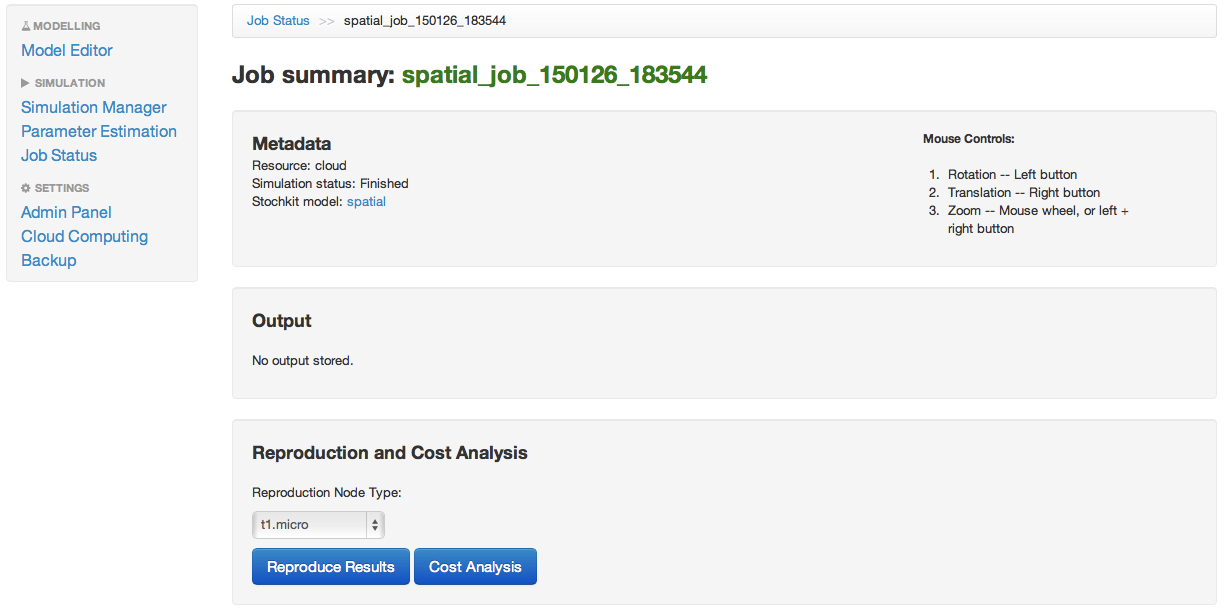
\includegraphics[scale=0.35]{T6_fig_reproduction1.png}
\caption{'Job summary' page - 'reproduction' available}
\label{fig:2}
\end{figure}

\newpage

\section{Cost Analysis}
To choose the right node type for job reproduction later, StochSS provides the possibility to analyze the time and money cost to run with different types of nodes. The results are plot for more intuitive comparison and best selection.

\subsection{An Example on Job Reproduction}
An example shown below will guide you on how to analyze the cost of reproduce an existing job.

\begin{figure}[!ht]
\centering
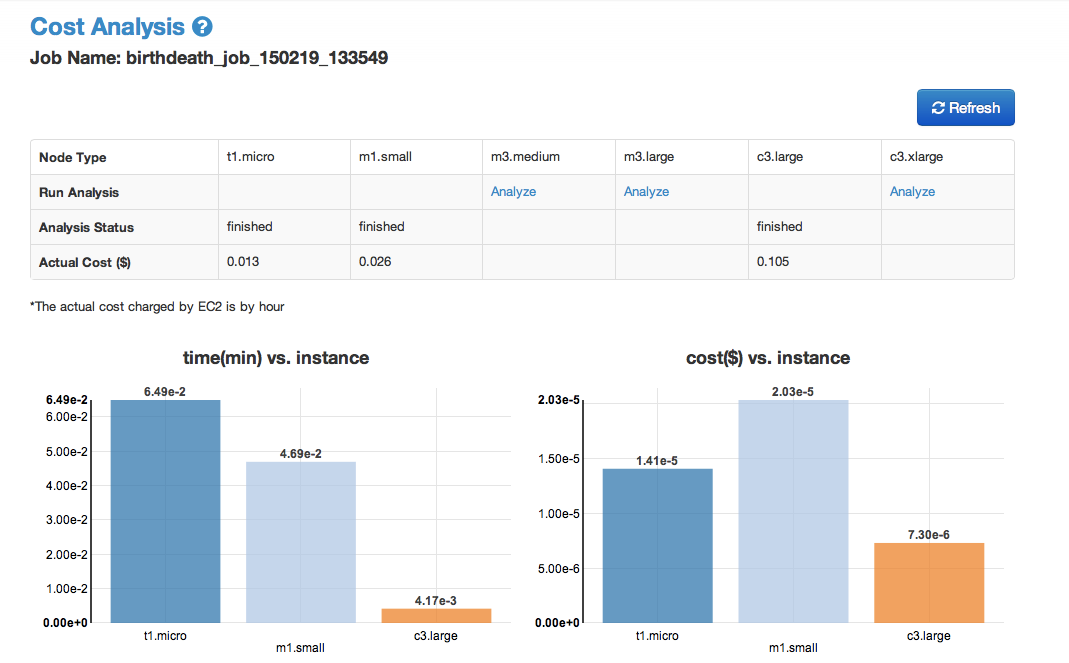
\includegraphics[scale=0.30]{T6_fig_costanalysis.png}
\caption{'Cost Analysis' page}
\label{fig:2}
\end{figure}

\begin{itemize}
\item \textbf{Navigate} to \textcolor{blue}{Job Status} page, which can be found by \textbf{clicking} \textcolor{blue}{'Job Status'} on the side bar.
\item \textbf{Click} the \textcolor{blue}{'view'} link of the job you would like to reproduce to go to the \textcolor{blue}{Job summary} page.
\item \textbf{Click} the \textcolor{blue}{'Cost Analysis'} button in the \textcolor{blue}{Reproduction and Cost Analysis} section.
\item \textbf{Click} the \textcolor{blue}{'Analyze'} button with the node type you would like to run and analyze. The page will auto refresh after the request is submitted and show its status of the analysis. If the analysis remaining to be \textcolor{blue}{'active'}, \textbf{click} the \textcolor{blue}{'Refresh'} button to refresh the status.
\item If the running is \textcolor{blue}{'finished'}, the time and money cost of running the job with the node type you chose will be plotted in the graph below for comparison.
\item \textbf{By default}, the cost of the job run for the first time will be recorded by cost analysis automatically, so that it doesn't need to rerun for the same instance type.
\end{itemize}


\end{document}
